%%%%%%%%%%%%%%%%%%%%%%%%%%%%%%%%%%%%%%%%%%%%%%%%%%%%%%%%%%%%%%%%%%%%%%%%%%%

\documentclass{standalone}

\usepackage{amsmath}
\usepackage{mathptmx}
\usepackage{pgfplots}
\usetikzlibrary{external}
\tikzexternalize{fortune100-linear}
\pgfplotsset{compat=1.15}

%% IEEE uses Times Roman font, so we'll default to Times.
%% These three commands make up the entire times.sty package.
\renewcommand{\rmdefault}{ptm}
\renewcommand{\ttdefault}{pcr}
\normalfont\selectfont

\begin{document}

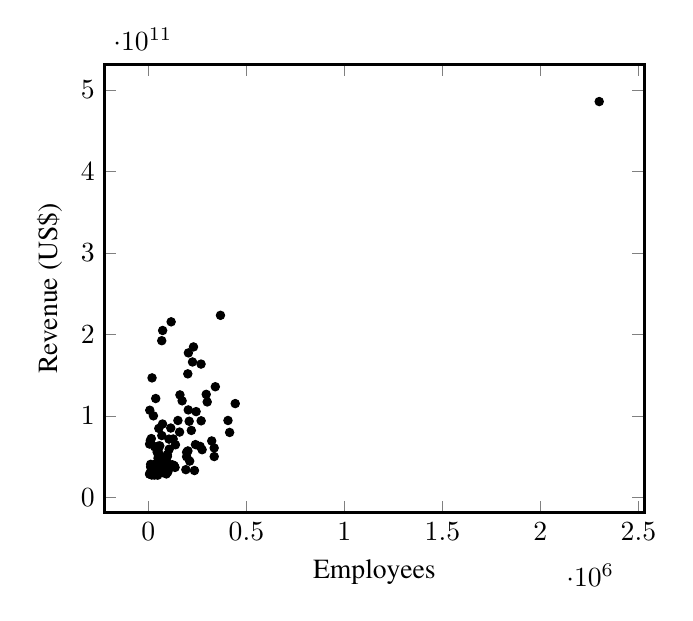
\begin{tikzpicture}
\tikzset{%%
  every mark/.append style={scale=1.0},%%
  scale=1.0%%
}
\pgfplotsset{%%
  every axis/.append style={font=\normalsize}%%
}
%%
\begin{axis}[%%
  axis line style=very thick,%%
  dotStyle/.style={mark size=1.5,black,mark color=black,mark=*,only marks},%%
  enlargelimits=true,%%
  %% x axis
  xlabel={\normalsize Employees},%%
  %% y axis
  ylabel={\normalsize Revenue~(US\$)}%%
]
%%
%%
\addplot[dotStyle] coordinates {
  (2300000, 485873000000)
  (367700, 223604000000)
  (116000, 215639000000)
  (72700, 205004000000)
  (68000, 192487000000)
  (230000, 184840000000)
  (204000, 177526000000)
  (225000, 166380000000)
  (268540, 163786000000)
  (201000, 151800000000)
  (18500, 146850000000)
  (341400, 135987000000)
  (295000, 126661000000)
  (160900, 125980000000)
  (37300, 121546000000)
  (172000, 118719000000)
  (300000, 117351000000)
  (443000, 115337000000)
  (203263, 107567000000)
  (7000, 107162000000)
  (243355, 105486000000)
  (25600, 100288000000)
  (406000, 94595000000)
  (150540, 94571000000)
  (269100, 94176000000)
  (208024, 93662000000)
  (72053, 90272000000)
  (114000, 85320000000)
  (53000, 84863000000)
  (219000, 82386000000)
  (159000, 80403000000)
  (414400, 79919000000)
  (68234, 76132000000)
  (14800, 72396000000)
  (126400, 71890000000)
  (105000, 71726000000)
  (9996, 70166000000)
  (323000, 69495000000)
  (5982, 65665000000)
  (240000, 65017000000)
  (138000, 64806000000)
  (58000, 63476000000)
  (49500, 63155000000)
  (264000, 62799000000)
  (31800, 62346000000)
  (335520, 60906000000)
  (106000, 59387000000)
  (49739, 58779000000)
  (274000, 58734000000)
  (201600, 57244000000)
  (44460, 55858000000)
  (195000, 55632000000)
  (51600, 54379000000)
  (96500, 52824000000)
  (56400, 52367000000)
  (97000, 50658000000)
  (51900, 50367000000)
  (335767, 50365000000)
  (195000, 50123000000)
  (73700, 49247000000)
  (49000, 48238000000)
  (56000, 48158000000)
  (210500, 44747000000)
  (100300, 41863000000)
  (11320, 40787000000)
  (30500, 40721000000)
  (122300, 40180000000)
  (34320, 40074000000)
  (68000, 39807000000)
  (41000, 39668000000)
  (83756, 39639000000)
  (125000, 39403000000)
  (131000, 39302000000)
  (95400, 38537000000)
  (50000, 38308000000)
  (55311, 37949000000)
  (11737, 37788000000)
  (34400, 37712000000)
  (30992, 37504000000)
  (12997, 37105000000)
  (136000, 37047000000)
  (114000, 36881000000)
  (88000, 36556000000)
  (43275, 36534000000)
  (191000, 34274000000)
  (56400, 33823000000)
  (235000, 33184000000)
  (70700, 32376000000)
  (34396, 31360000000)
  (98800, 31353000000)
  (70580, 30737000000)
  (9000, 30390000000)
  (12157, 30347000000)
  (91584, 30109000000)
  (25000, 29318000000)
  (91500, 29003000000)
  (5646, 28799000000)
  (17048, 27638000000)
  (30900, 27625000000)
  (47300, 27519000000)
};
\end{axis}
\end{tikzpicture}

\end{document}
